\section{Design}
TODO:
We use an agent for this target group

In order to measure the enjoyability of a location-based game (LBG) with a game activity as the navigational method between POIs, we developed a LBG. The game takes place in Aalborg, Denmark and the points of interest (POIs) are three street art paintings\cite{streetart}. The game makes players walk between the three POIs on a route with a total length of 1.8km and a distance of 0.9km between POIs (see Figure \ref{FinalRoute}). Due to requirements from the method of the experiment as described in (INSERT REFERENCE TO METHOD SECTION), the particular route was chosen on the basis of it having a close to equal amount of intersections in the road between POIs as well as a close to equal distance between the POIs.

\begin{figure}[hbtp]
\centering
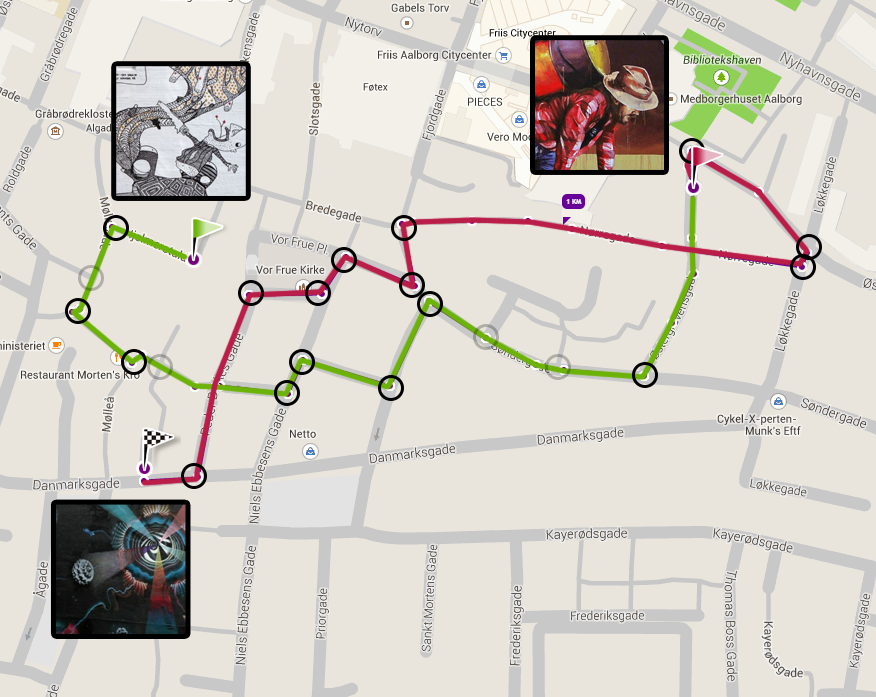
\includegraphics[scale=0.3]{Pics/FinalRoute.png}
\caption{The route between the three street art paintings.}
\label{FinalRoute}
\end{figure}

\subsection{Choice of Navigational Game Activity}
In the process of designing the navigational game activity using landmarks, four initial designs were created as paper prototypes and one was chosen to be used in the game on the basis of three initial tests of the designs. The tests were done using within-subjects design, meaning that each group of participants used a specific navigational game activity for each quarter of the route. The purpose of the tests was to determine which game activity the participants found most enjoyable, based on short semi-interviews conducted between game activities as well as after trying all four activities. The participants of each test were a child in the age group of 8-11 years and the child's parent. As the initial designs were paper prototypes with a focus on the navigation, it must be noted that elements of LBGs such as a feedback system, a narrative, activity at POIs, and learning were not a part of the experience in these initial tests.

When designing the four navigational game activities, inspiration was taken from popular children's games, since they are familiar to most children, causing a lower learning curve for the families. Similar game activities were also found in other LBGs, giving inspiration for how they should be used in a LBG. Three navigational game activities were made as variations of matching card games such as \textit{Concentration}\cite{childrensGames}. In these types of games, players specify two or more cards that are alike, among a set of cards, and the goal is typically to be the player with the most matches in the end. In Team Exploration\cite{GamingOnTheMove}, players match pictures in the virtual space to landmarks in the physical space and progress in the game by specifying which pictures belong to certain areas of a map. Similarly, players are given pictures of landmarks in our three matching game activities; \textit{Simple Matching}, \textit{Order Matching}, and \textit{Memory Matching}.

For all four game activities, local landmarks are used to help players choose directions at decision points, and route marks are used along streets to confirm to players that they are walking in the correct direction. In Simple Matching, players are given a set of potential landmarks, where only one of them is a true landmark in their current location. When they spot or match the landmark that is shown on the picture, they go to its position and start matching the next set of pictures. This prototype proved to be the easiest of the four and most participants found it to be uninteresting due to its lack of challenge. Order Matching is very similar to Simple Matching, and the only difference is that players have to specify the order in which the presented landmarks occur in the vicinity of their current position. Furthermore, in this design only landmarks that are in the vicinity are presented to the player. The intention of this design was to make the matching task more challenging, however observations and interview answers showed that participants still did not find it to be very challenging. Observations also showed that participants sometimes walked back in the direction they came from to get the order right. However for this design, it was also seen that the participants collaborated and communicated more in general. In Memory Matching, collaboration and communication between participants is encouraged even more by removing the ability to view the pictures while navigating, and only presenting the pictures to participants quickly. When participants then reach the last picture in the set, they are asked to specify the order of landmarks encountered. This design showed the most collaboration and communication between participants and 





 , where players  and CityTreasure\cite{botturi2009city}. 

\subsection{Lost on Earth}
